\graphicspath{{chapters/notes/05/images}}
\chapter{Tumor Evolution Studies via NGS data}

\section{Tumour evolution}

	\subsection{Introduction}
	To be fully able to treat cancer it is important to understand what are the somatic events that occur during tumor genesis and evolution and when they arise.
	Cancer cells accumulate mutations due to both cell division and toxic agents like radiations or UV light.
	These mutations are maintained by the cell and lead to clonal expansion.
	Cancer could then originate or evolve through an arbitrary number of driver mutations that could, for example, activate an oncogene or disrupt some molecular pathways.

		\subsubsection{Typical traits of cancer}
		Typical traits of cancer are:

		\begin{multicols}{2}
			\begin{itemize}
				\item Cancer is a dynamic disease: tracking its evolution if fundamental.
				\item During the course of disease, cancers generally become more heterogeneous, which is often related to treatment resistance.
				\item The bulk tumour includes a diverse collection of cells harbouring distinct molecular signatures with differential levels of sensitivity to treatment.
				\item This heterogeneity might result in a non-uniform distribution of genetically distinct tumour-cell sub-populations across and within disease sites (spatial heterogeneity) or temporal variations in the molecular make-up of cancer cells (temporal heterogeneity).
			\end{itemize}
		\end{multicols}

		\subsubsection{Tumour boards}
		Tumour boards are teams of specialists that follow a cancer patient through treatment.
		They collect data and suggest course of actions during the illnesses and can teach new doctors how to manage difficult cases.

	\subsection{Heterogeneity}
	Every site of the genome with somatic mutations is going to be differentially represented in tumour samples.
	Heterogeneity drives cancer resistance and is a great obstacle in treatment.
	Therefore, an accurate assessment of tumour heterogeneity is essential for the development of effective therapies.
	Emerging techniques to study with considerable potential to dissect the complex clonal architecture of cancers heterogeneity are:

	\begin{multicols}{2}
		\begin{itemize}
			\item Multi-region sequencing.
			\item Single cell sequencing.
			\item Analysis of autopsy samples.
			\item Longitudinal analysis of liquid biopsy samples.
		\end{itemize}
	\end{multicols}

	However, techniques to study tumour heterogeneity are hindered by intra-patient heterogeneity, which can be spatial or temporal.
	Figures \ref{fig:hetero} describes tumour heterogeneity.

	\begin{figure}[H]
		\centering
		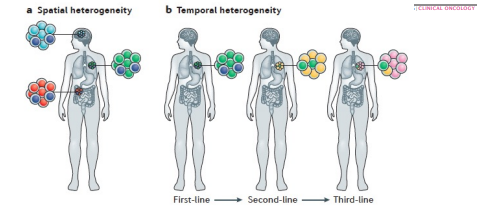
\includegraphics[width=0.7\textwidth]{heterogeneity.png}
		\caption{a) Spatial heterogeneity denotes an uneven distribution of cancer subclones across different regions of the primary tumour and/or metastatic sites. b) Temporal heterogeneity refers to variations in the molecular make-up of a single lesion over time, either as a result of natural progression of the tumour or as a result of exposure to selective pressures created by clinical interventions. Colours denote the presence of subclones with different genetic features.}
		\label{fig:hetero}
	\end{figure}

		\subsubsection{Temporal heterogeneity}
		Temporal heterogeneity refers to the change in time of a single tumour mass.
		This can happen naturally or under particular selective pressures.

		\subsubsection{Spatial heterogeneity}
		Spatial heterogeneity describes different independent tumour masses that can be found in patients which share certain cells while having a unique genetic make-up.

	\subsection{Type of evolutions}
	It could be possible that some cells positively respond to treatment and others not, creating a heterogeneous population in the mass.
	The features of this set of cells changes over time.
	This evolution happens either because the new population replaces the older, or there's a branching and the tumour mass becomes heterogeneous.
	Moreover a metastatic mass could have a monoclonal (from one mass) or polyclonal (from different masses) origin.

	\begin{figure}[H]
		\centering
		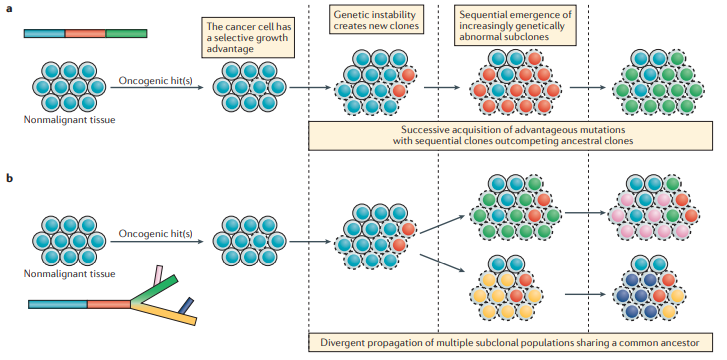
\includegraphics[width=0.7\textwidth]{branching.png}
		\caption{ a) everything branches out from the monoclonal origin, but b) polyclonal origin, independent metastatic processes. Cells from independent lesions meet and form a highly diverse metastatic tumour.}
		\label{fig:branching}
	\end{figure}

		\subsubsection{Linear evolution}
		Sequential genetic alterations confer a fitness advantage such that successive generations are able to out compete the preceding clones, which lack this fitness advantage.
		Surviving dominant clones harbour the ancestral mutation.

		\subsubsection{Branched evolution}
		Multiple genetically distinct populations can emerge from a common ancestral clone, with certain subclonal populations diverging from the common ancestor before others.


	\subsection{Treatment resistance}

	\begin{figure}[H]
		\centering
		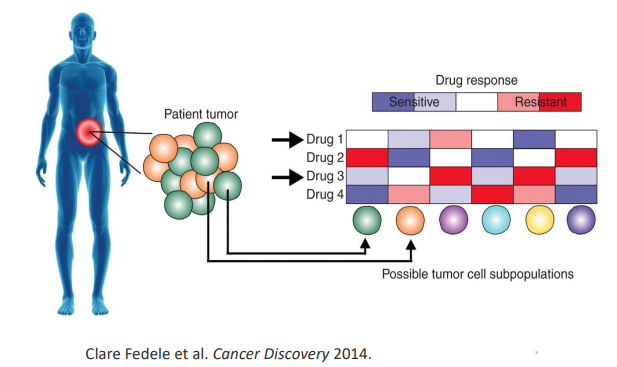
\includegraphics[width=0.6\textwidth]{treatment.png}
		\caption{Certain cells of the tumour mass respond to treatment and some don't. Red cells are resistant to the drug, while blue cells are sensitive to it.}
		\label{fig:treatment_resistance}
	\end{figure}

	Tumour resistance to treatment can be encoded in the original cells or can be driven by the treatment.
	Figure \ref{fig:response} depicts the processes that drive resistance that originates from treatment.
	This can be due to the selection of clones that provide resistance or the transformation of clones under treatment pressure.

	\begin{figure}[H]
		\centering
		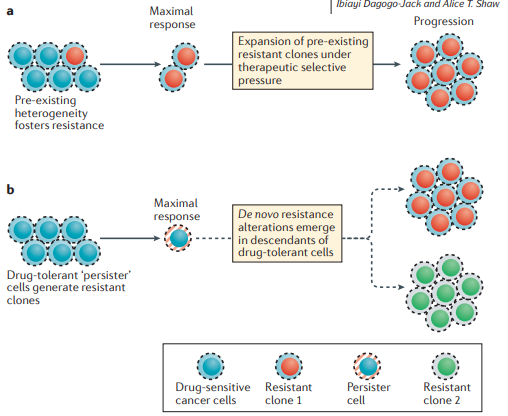
\includegraphics[width=0.7\textwidth]{response.png}
		\caption{ Tumor cells evolution driven by treatment.}
		\label{fig:response}
	\end{figure}

		\subsubsection{Primary resistance}
		Pre-existing heterogeneity fosters resistance.
		Only susceptible cells die and resistant cells continue dividing, allowing the tumour to regrow.
		An high tumour mass will be visible.

		\subsubsection{Acquired resistance}
		Drug-tolerant, persistent cells generate resistant clones.
		At the time of diagnosis there are no markers of the resistance alteration because it is developed afterwards.
		The resistant cells will form over time new tumours not responding to the drug.

\section{Using NGS data to uncover tumour evolution}

	\subsection{Introduction}
	A tumour is a collection of multiple independent lesions.
	Sequencing can be used to obtain a representation of tumour burden and of the features of all of the different areas.
	In order to study tumor evolution common and private lesions across multiple samples from the same individual can be used to reconstruct the evolutionary path.
	Data from multiple individuals can be used, selecting the most clonal lesion, to build a common clonal evolution map.
	From this type of data it has been found, for example that in prostate cancer if CHD1 is mutated, then a subsequent PTNEN mutation is found.
	The interest is on finding which lesions occurred first and which is the model that fits better the data.
	In particular when dealing with tumour data there is a need to take into account:

	\begin{multicols}{2}
		\begin{itemize}
		\item Intra tumor heterogeneity.
		\item Inter tumor/intra patient heterogeneity.
		\item Inter-patient heterogeneity.
		\item Clinical/treatment relevance.
		\item Time dependency.
		\item Admixture DNA (tumor purity).
		\end{itemize}
	\end{multicols}

	This characteristics, if properly investigated, can provide insightful hints during the analysis.

	\subsection{Admixture}
	A sample coming from a patient's tissue contains multiple cell types.
	So a sample will never be composed only of cancer cells.
	DNA admixture refers to the percentage of cells that are not tumoral.
	Purity, instead, is the percentage of cancer cells in a sample.
	It is computed as:

	$$Pur = 1-Adm$$

	A particular lesion is clonal if all tumour cells harbour it.
	If only a portion of cells harbour it it is subclonal.
	Purity and admixture can be used to distinguish between clonal and subclonal lesions.

	\subsection{Informative SNPs}
	SNPs can be exploited to characterize tumour evolution.
	Informative SNPs are heterozygous SNPs: the allelic fraction can be counted and the proportion of reads supporting the alternative base can be assessed.
	The allelic fraction will change for somatic events that involve the genomic locus of a particular SNP, allowing to detect them.
	This is represented in \ref{fig:af_properties}.
	For example in a deletion the allelic fraction of a heterozygous SNP will change from $0.5$ to either $0$ or $1$.
	In particular when selecting informative SNPs to design an assay is important to consider their MAF together with data from databases like dbSNP to select the one that are most probable to are in an heterozygous genotype.

	\begin{figure}[H]
		\centering
		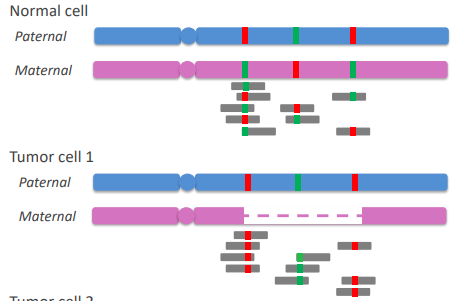
\includegraphics[width=0.5\textwidth]{af_properties.png}
		\caption{Thanks to the presence of informative SNPs is easy to detected the loss of an allele in the tumour cell.}
		\label{fig:af_properties}
	\end{figure}

	\subsection{Beta value}
	When dealing with non pure samples the $\beta$ value needs to be introduced to uncover events concerning informative SNPs.
	This is because the allelic fraction signal will change based on the purity: in fact when only some cells in the sample are from a tumour the allelic fraction distribution will have two peaks.
	$\beta$ is the percentage of neutral reads, or the number of reads that can be coupled, one with the reference base and one with the alternative, over the total number of reads at that SNP.
	In particular:

	\begin{multicols}{2}
		\begin{itemize}
			\item $\beta = 1$ both alleles equally represented.
			\item $\beta = 0$ only one allele represented.
		\end{itemize}
	\end{multicols}

	The more $\beta$ is far from $1$, the more the sample is admixed or the more the lesion is clonal.
	Moreover $Nref$, the percentage of the reference base in the non-deleted allele can be introduced.
	Figure \ref{fig:b_af_purity} links together the concepts of $\beta$, sample purity and allelic fraction.

	\begin{figure}[H]
		\centering
		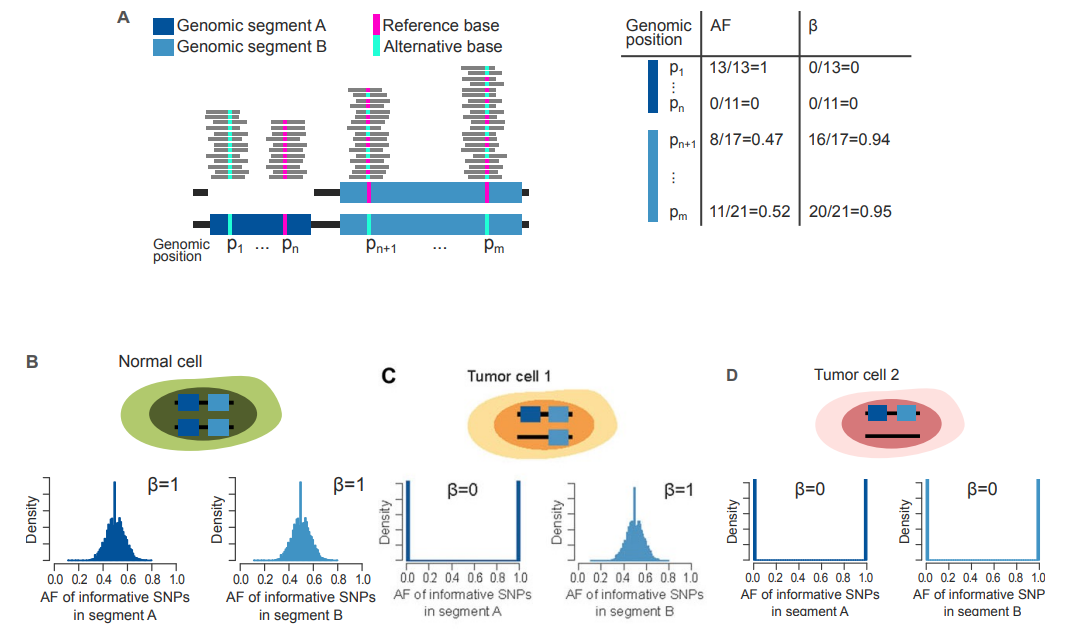
\includegraphics[width=0.8\textwidth]{a.png}
		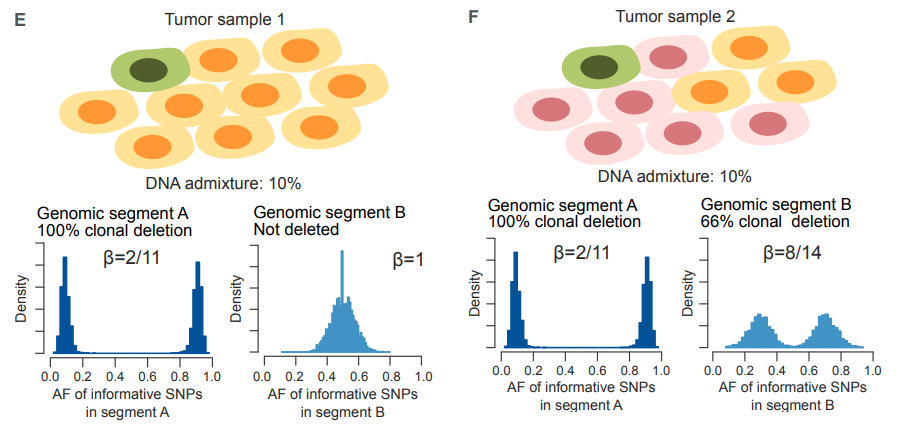
\includegraphics[width=0.8\textwidth]{b.png}
		\caption{A)Example of the allelic fraction (AF) and beta ($\beta$) computed in five genomic positions ($p_1$ to $p_m$).
			Positions $p_1$ to $p_n$ are within a hemizygous deleted genomic segment A, while genomic positions $p_{n+1}$ to $p_m$ lie within a wild type genomic segment B.\\
			B-D) Examples of a normal cell and two different tumor cells.
			Tumor cells 1 and 2 differ for the status of genomic segment B.
			Histograms below cell cartoons report the expected distribution of the allelic fraction of SNPs in genomic segments A and B together with the associated beta values.\\
			E-F) Examples of two different tumor samples.
			Tumor sample 1 includes one normal cell and nine tumor cells with deleted genomic segment A and wild type genomic segment B.
			Tumor sample 2 differs from tumor sample 1 in the presence of six tumor cells with a hemizygous deletion of genomic segment B.
			Expected distribution of the AF of informative SNPs together with estimated beta are depicted below each tumor sample cartoon.}
		\label{fig:b_af_purity}
	\end{figure}

		\subsubsection{Computing beta}
		$\beta$ can be computed for each genomic segment $S$:

		\begin{multicols}{2}
			\begin{enumerate}
			\item Compute the observed distribution of the $AF$ of informative SNPs in the genomic segment $S$.
			\item Find the values of $\beta$ and $Nref$ such that the expected distribution of the $AF$ matches the observed $AF$.
			\item Compute uncertainty around $\beta$ as a function of:
				\begin{enumerate}
				\item The mean coverage of $S$.
				\item The number of informative SNPs in $S$.
				\end{enumerate}
			\end{enumerate}
		\end{multicols}


		\subsubsection{Effect of coverage on beta}
		The mean coverage of an experiment impact the accuracy of $\beta$.
		The more deep a sequencing is more two close peaks of $AF$ can be distinguished.
		This is especially important when $\beta$ is close to $0$.
		An example of the effect of coverage on $\beta$ is shown in figure \ref{fig:cov_beta}.

		\begin{figure}[H]
			\centering
			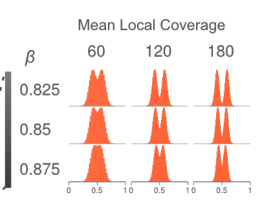
\includegraphics[width=0.4\textwidth]{beta.png}
			\caption{2X experiment: on average there are $2$ reads per gene.
				It is easy to not recognize the correct distribution.\\
				10X experiment: it is easy to recognize the correct distribution.
				The process becomes more difficult for a tumour sample.
				This image shows how the higher the sequencing depth, the more the two peaks of the distribution are distinguishable.}
		\label{fig:beta}
		\end{figure}

	\subsection{Estimates of global and local admixture}
	To understand how to determine the admixture two samples will be considered.

	\begin{figure}[H]
		\centering
		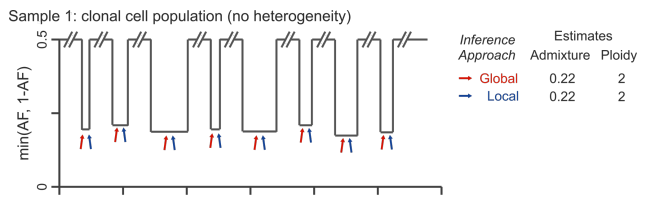
\includegraphics[width=0.7\textwidth]{sample1.png}
		\caption{In the clonal cell population how much the distribution deviates from AF is the same globally and locally.}
		\label{fig:sample1}
	\end{figure}

	In sample one (figure \ref{fig:sample1}) a clonal cell population is represented.
	So there is no heterogeneity.
	On the $x$-axis there are the genomic coordinates indexed by informative $SNP$, on the $y$-axis the $AF$.
	Drops in the allelic fraction represent lesions, and it can be seen how all drops are of the same length on the $y$ axis.
	This means that the amount of DNA loss or gain is identical in all of this drops.
	This means that the level of admixture remains constant over all the sample and is the same both globally and locally.

	\begin{figure}[H]
		\centering
		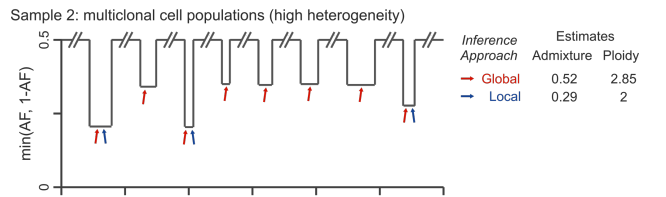
\includegraphics[width=0.7\textwidth]{sample2.png}
		\caption{This sample harbours heterogeneity: the global and local values of admixture are different. A global value is relative to tumor purity, while local to clonality.}
		\label{fig:sample2}
	\end{figure}

	In sample two (figure \ref{fig:sample2}) a multiclonal cell population is represented.
	Multiclonality is characterized by different depth of lesions.
	In fact the depth of the drop is proportional to the number of cells that carry that lesion.
	So, in this case the global admixture refers to tumor purity, while the local one to the clonality of the lesion in the diseased cell population.

		\subsubsection{Estimates of DNA admixture}
		The estimates of global and local admixture can be combined together with the $\beta$-value and the log2 ratio, as is depicted in figure \ref{fig:2D}.
		The log2 ratio is computed as:

		$$\log_2\frac{tumour_{samples}}{normal_{samples}}$$

		\begin{figure}[H]
			\centering
			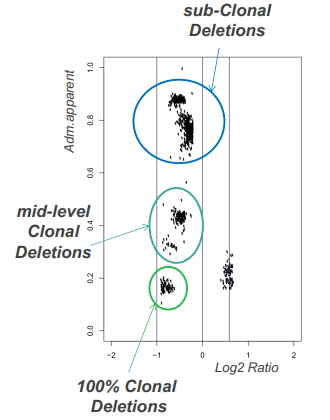
\includegraphics[width=0.5\textwidth]{adm.png}
			\caption{Each dot is a genomic segment and different clusters are visible. Lower clusters are used to determine the admixture while the other represent subclonal cells. Close points probably represents lesions that happened close in time.}
			\label{fig:2D}
		\end{figure}

		On the $x$ axis the log2 ratio is measured while on the $y$ the apparent admixture, which is proportional to $\beta$.
		The log2 ratio allow to interpret information about every segment in the genome when coupled with $\beta$.
		Apparent admixture is computed as:

		$$Adm.apparent = \frac{\beta}{2-\beta}$$

		And associates an apparent DNA admixture to each monoallelic deletion.
		The clonality is computed from the apparent admixture and the global one:

		$$Clonality = \frac{1-Adm.apparent}{1-Adm.global}$$

	\subsection{PR-2741 - an example}
	Figure \label{fig:adm} depicts data of a real case of prostate cancer in which a clear drop in coverage in region $2$ of the $5th$ chromosome, while region $1$ and $3$ have equal coverage can be seen.
	The DNA present in region $2$ could come either from admixing cells or from cells that do not have the deletion.
	Looking at the allelic fractions of region $1$, $2$ and $3$, both from the tumour and the match normal normal sample more or less the same two modes of distribution are observed.
	In the tumour sample in fact the expected peaks at $0$ and $1$ are not observed.
	This could be due to signal coming from intervening normal cells, that bring the modes to the center, or due to subclonality events.
	It is clear how a subclonality event could be uncovered through a lesion with admixture.

	\begin{figure}[H]
		\centering
		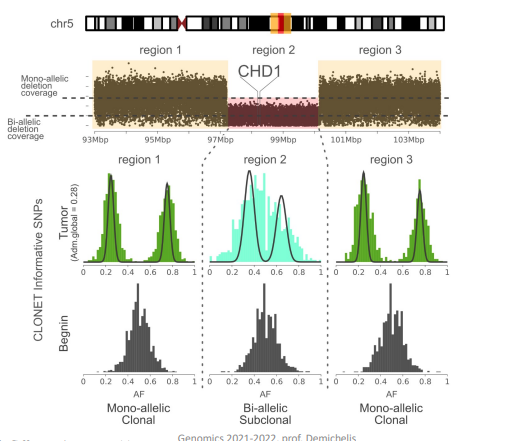
\includegraphics[width=0.7\linewidth]{PR_2741.png}
		\caption{The distribution of heterozygous SNPs in benign cells is peaked at $0.5$, while two modes in tumour cells are observed. The distance between the two modes is equal in $1$ and $3$. In the middle the two modes are moving towards the center, suggesting that the deletion is not likely $100\%$ clonal or it is clonal and shifts is due to lack of deletion in $1$ and $3$}
		\label{fig:adm}
	\end{figure}
